\section{Beispiele}

\subsection{CppUnit}
\lstinputlisting{source/CppUnit/AuthorTest.cpp}
\newpage

\subsection{Doxygen}
\begin{tabular}{l l}
	\textbf{Eclipse Einstellungen} & \textbf{Eclipse-Plugin}\\
	\tabbild[width=9cm]{images/doxygen_advanced.png} & \tabbild[width=9cm]{images/doxygen_basic.png}\\
\end{tabular}
\newpage
\begin{multicols}{2}
	\lstinputlisting[linewidth=11cm]{source/Doxygen/doxygenbsp.c}	
	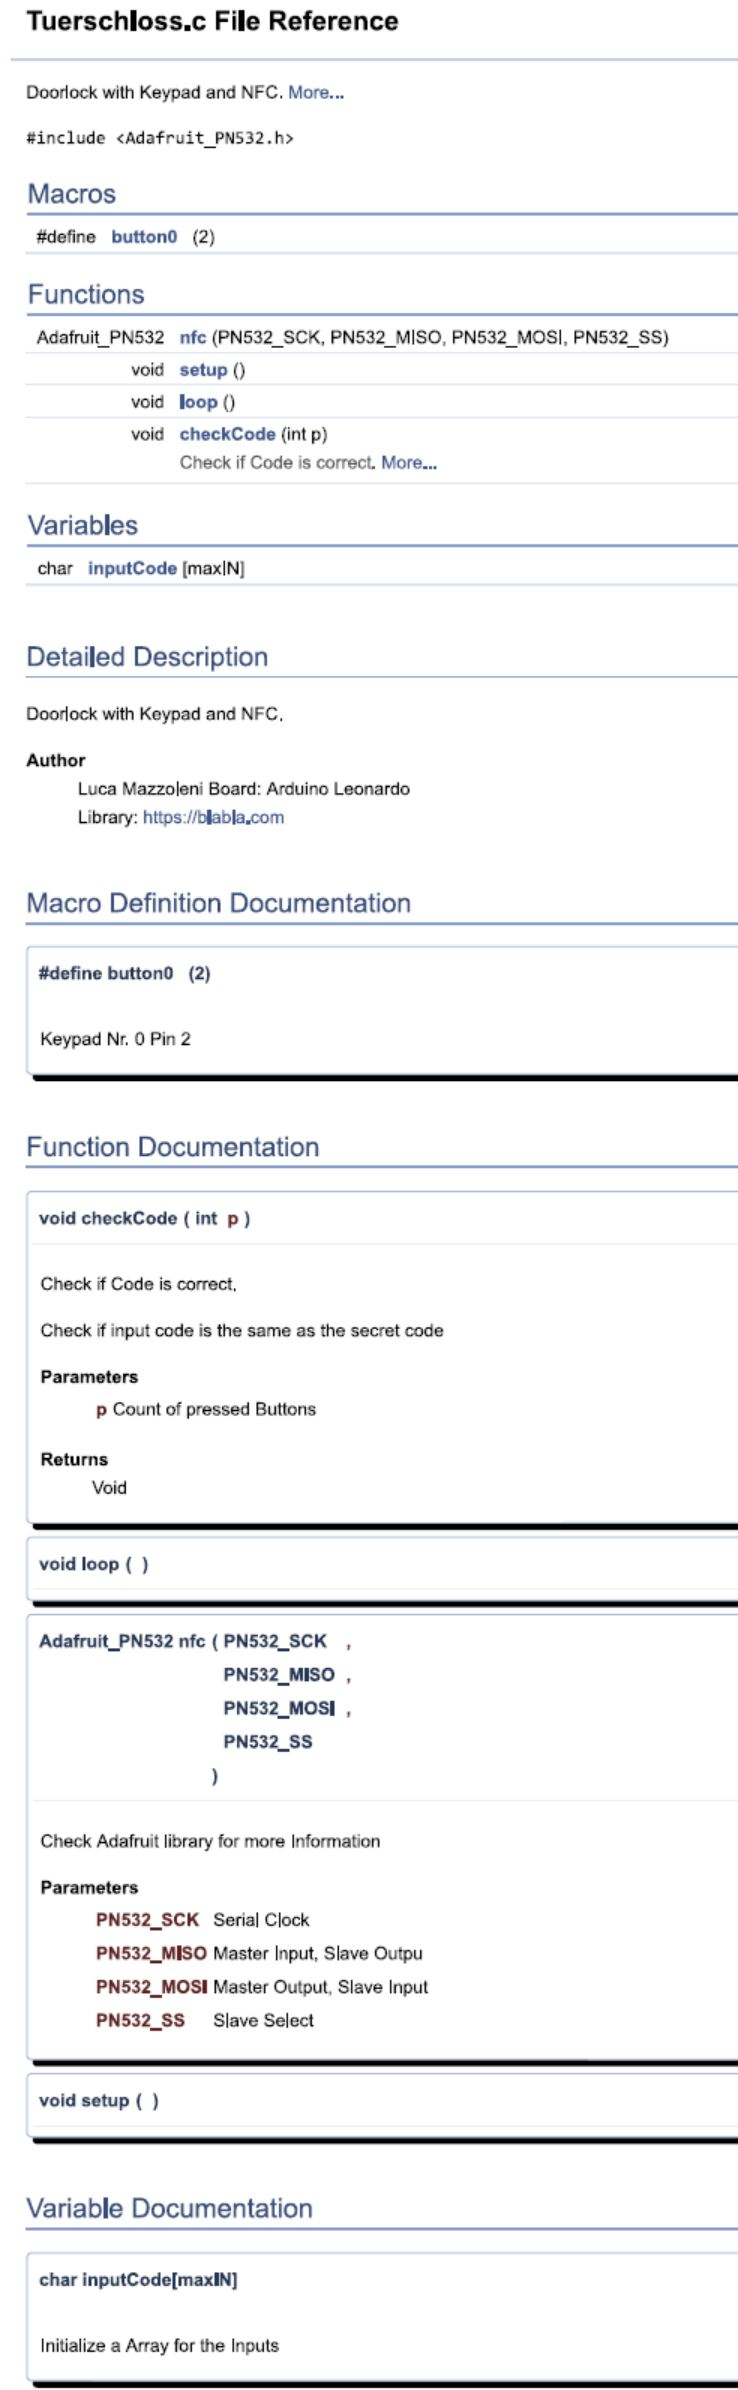
\includegraphics[width=8cm]{images/html.JPG}
\end{multicols}	
\pagebreak

\subsection{Qt}
\subsubsection{Hello World}
\lstinputlisting{source/Qt/hello_world.cpp}
\subsubsection{QWidgets}
\begin{tabular}{c c}
	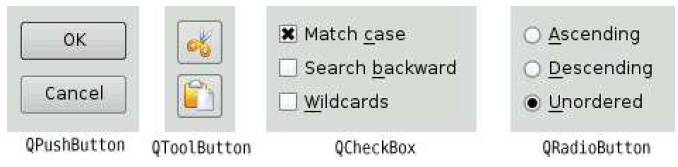
\includegraphics[width=9cm]{images/button_1.png}& 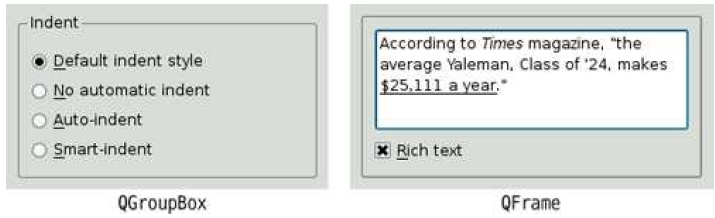
\includegraphics[width=9cm]{images/button_2.png}\\
	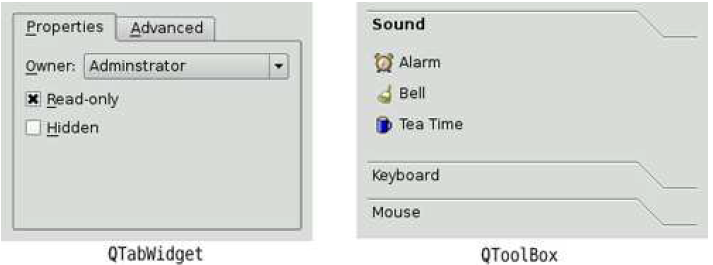
\includegraphics[width=9cm]{images/button_3.png}& 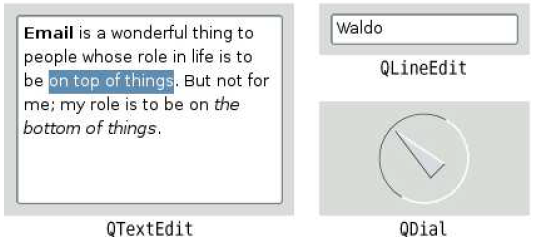
\includegraphics[width=9cm]{images/button_7.png}\\
	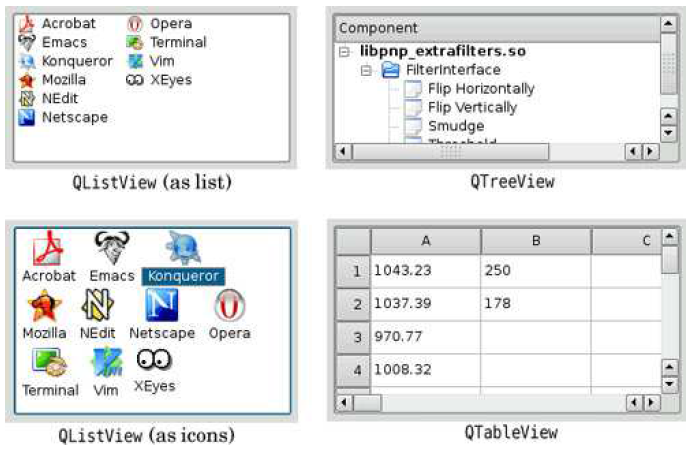
\includegraphics[width=9cm]{images/button_4.png}&
	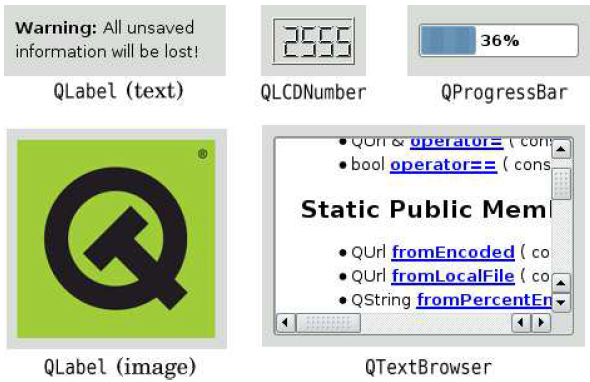
\includegraphics[width=9cm]{images/button_5.png}\\
	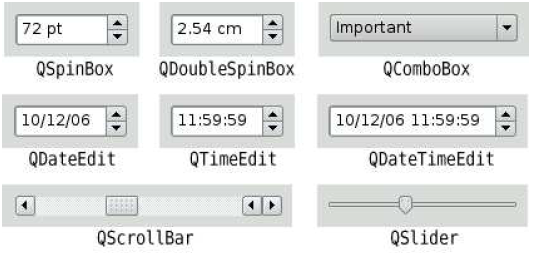
\includegraphics[width=9cm]{images/button_6.png}&
	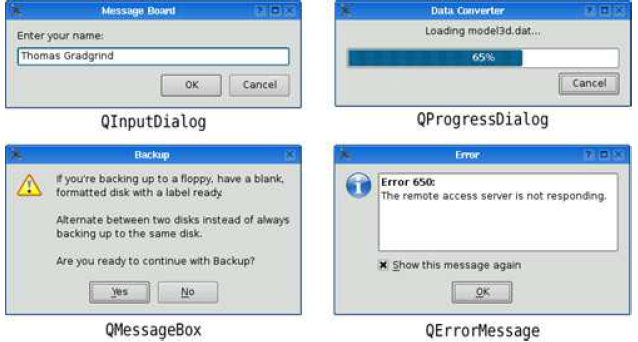
\includegraphics[width=9cm]{images/button_8.png}\\
\end{tabular}
\subsubsection{QBrush}
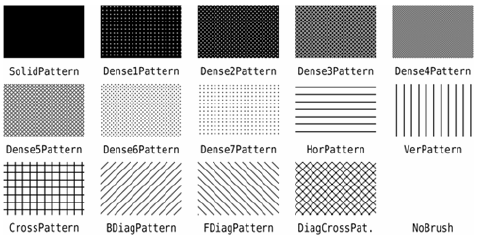
\includegraphics[width=9cm]{images/brush.png}

\subsubsection{QPainter draw-Methoden}
\begin{tabular}{c c}
	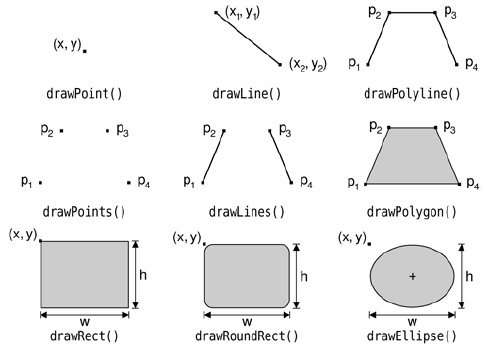
\includegraphics[width=9cm]{images/draw_1.png}& 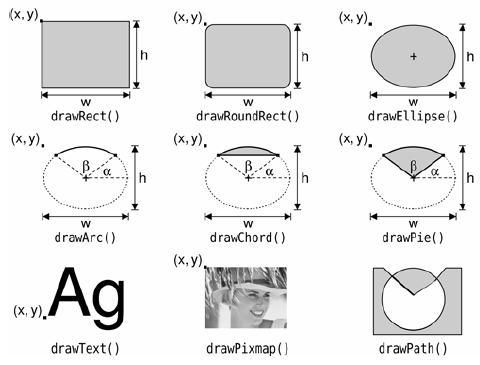
\includegraphics[width=9cm]{images/draw_2.png}\\
\end{tabular}
\subsubsection{QPen}
\begin{tabular}{c c}
	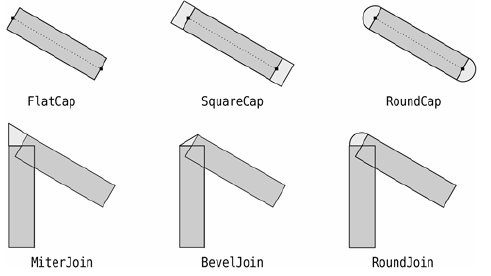
\includegraphics[width=9cm]{images/pen_1.png}& 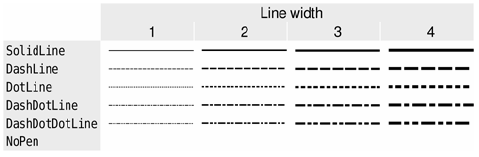
\includegraphics[width=9cm]{images/pen_2.png}\\
\end{tabular}
\newpage
\subsubsection{Temperaturwidget}
\textbf{main.cpp}
\\
\lstinputlisting{source/Qt/main.cpp}
\textbf{temperaturwidget.h}
\\
\lstinputlisting{source/Qt/temperaturwidget.h}
\newpage
\textbf{temperaturwidget.cpp}
\lstinputlisting{source/Qt/temperaturwidget.cpp}